\chapter{Methodology}
\section{Operations Research Model}
\emph{in silico analyses} attempts can be introduced here in more detail.

\subsection{Background Information}
The genome-scale metabolic network model (GEM) is one of the fundamental frameworks used in metabolic engineering. Fig.~\ref{figure-metabolic-networks} shows two differently constructed network graphs that represent relations of metabolites, intermediate or end products, with their metabolic reactions for a particular metabolism: Homo Sapien. Fig.~\ref{figure-metabolic-centric} graph nodes are the metabolites, graph edges are the reactions, whereas the graph nodes and edges represent vice versa in Fig.~\ref{figure-reaction-centric}. 

\begin{figure}[!ht]
	\centering
	\begin{subfigure}{0.5\textwidth}
		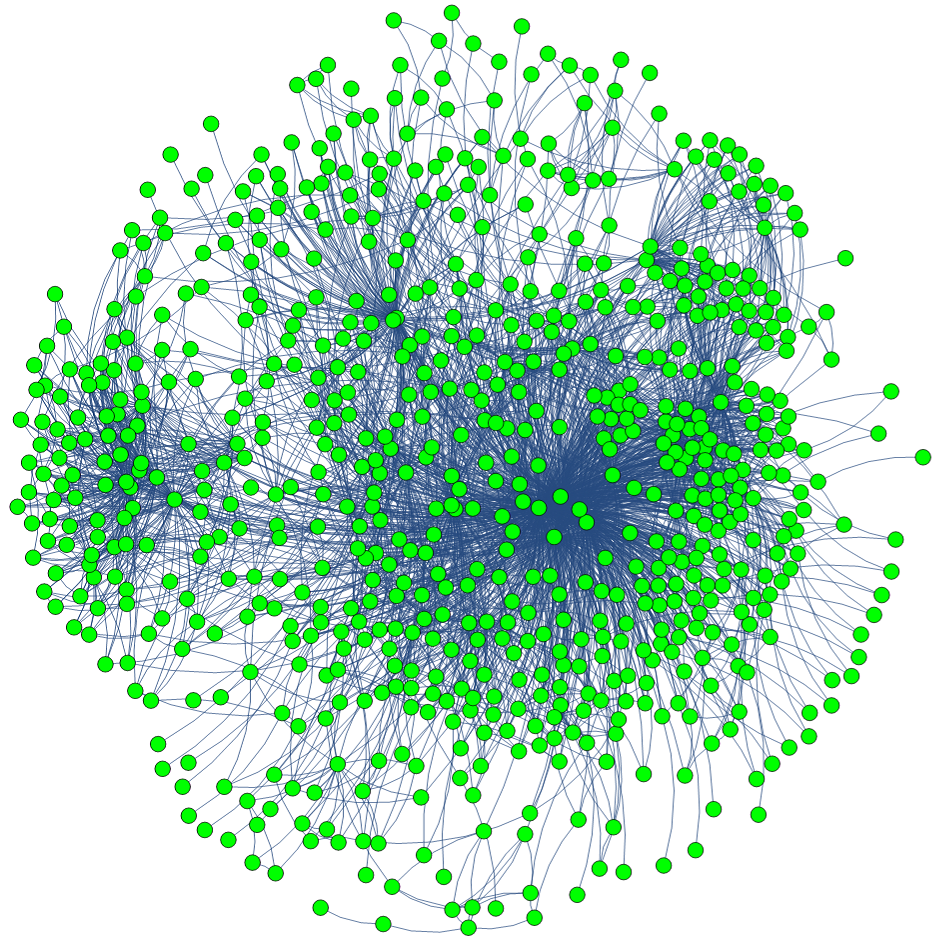
\includegraphics[width=1\linewidth]{../images/methodology-ORmodel-metabolic_centric_network.png}
		\caption{Metabolic-centric Network}
		\label{figure-metabolic-centric}
	\end{subfigure}\hfill% or \hspace{5mm} or  \hspace{0.3\textwidth}
	\begin{subfigure}{0.5\textwidth}
		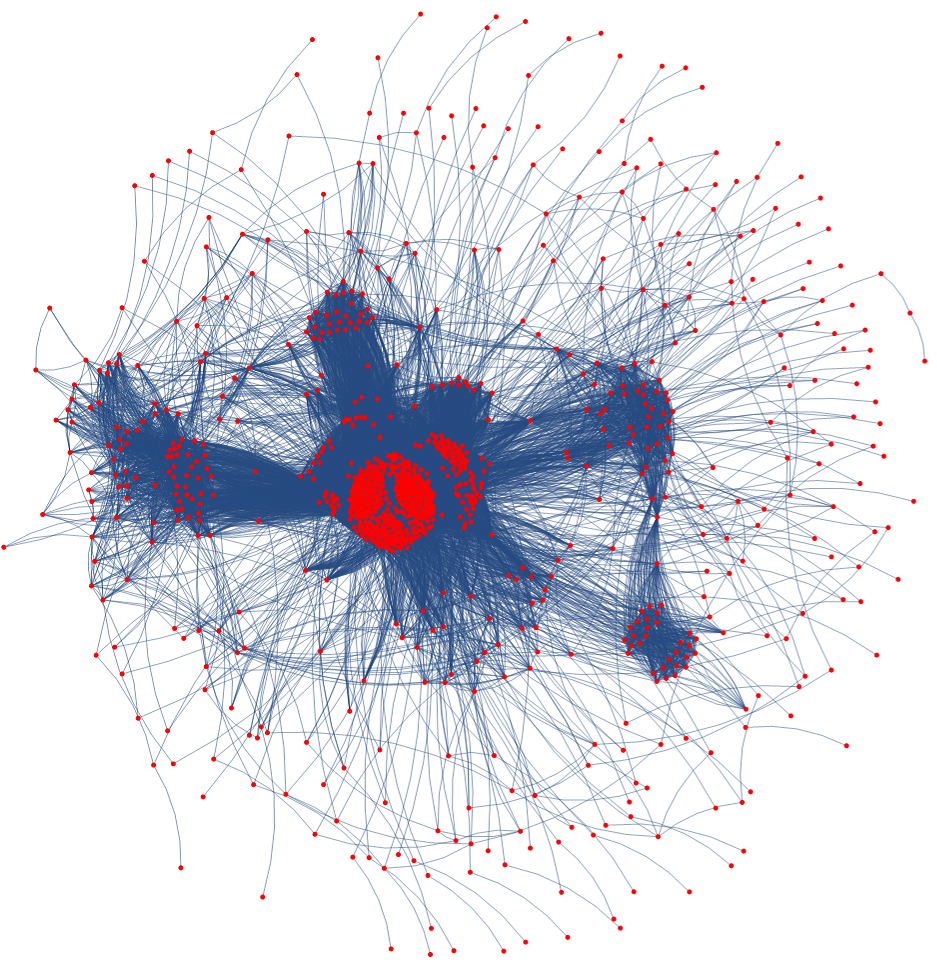
\includegraphics[width=1\linewidth]{../images/methodology-ORmodel-reaction_centric_network.png}
		\caption{Reaction-centric Network}
		\label{figure-reaction-centric}
	\end{subfigure}
	\caption{Network Representations for Homo Sapiens Metabolic Model}
	\label{figure-metabolic-networks}
\end{figure}

Various tools are being used to analyze reconstructed GEMs to understand how the metabolic networks function within their relevant system objectives and adapt robustly to conditional changes in their environments~\cite{KIM, HAO}. One of the commonly used tools is Flux Balance Analysis (FBA). It is a constraint-based modeling approach used by metabolic engineers to simulate microbial metabolisms\textemdash can be applied to biochemical-reaction networks containing the chemical transformations and flux changes in that particular network~\cite{KAUFFMAN2003491, PRICE2004}.

Although the networks shown in Fig.~\ref{figure-metabolic-networks} do not contain any information about the directionality or the degree of effectiveness of reactions to the system, the set of rules take place in networks can be represented in more detail and stoichiometrically by an m-by-r matrix formulation: Stoichiometric Matrix, $S$, whereas its column elements represent reactions play a role in the chemical transformation, and its row elements represent metabolites as
\begin{equation} \tag{1}
	S =  \begin{bmatrix} 
		s_{11} & s_{12} & \dots  & s_{1r}\\
		s_{21} & s_{22} & \dots  & s_{2r}\\
		\vdots & \vdots &\ddots & \vdots \\
		s_{m1} & s_{m2} & \dots & s_{mr} 
	\end{bmatrix}=(s_{ij})\in \mathbb{Z}^{mxr},
	\label{stoichio}
\end{equation}
while one can express the fluxes in a one-dimensional array: Flux Vector, $V$ as 
\begin{equation} \tag{2}
	V = \begin{bmatrix} 
		v_{1} \\
		v_{2} \\
		\vdots \\
		v_{r}
	\end{bmatrix}=(v_{i})\in \mathbb{R}.
	\label{solutionvector}
\end{equation}
$V$ contains flux exchange values for the corresponding reactions in the system and gives information about the flux distribution; hence those can be both positive and negative real numbers. Definition of a mass balance ($S.V=0$) constraint in the FBA enables us to analyze the metabolic network operations in a steady-state~\cite{KAUFFMAN2003491,PRICE2004}.
%(resulting steady state vectors/resulting optimized solution vectors)
\begin{equation} \tag{3}
	S.V = \begin{bmatrix} 
		s_{11}v_{1} + s_{12}v_{2} + \dots + s_{1r}v_{r} \\
		s_{21}v_{1} + s_{22}v_{2} + \dots + s_{2r}v_{r} \\
		\vdots \\
		s_{m1}v_{1} + s_{m2}v_{2} + \dots + s_{mr}v_{r} 
	\end{bmatrix}=
	\begin{bmatrix} 
		0 \\
		0 \\
		\vdots \\
		0
	\end{bmatrix}.
	\label{massbalanceconstraint}
\end{equation}
The higher amount of metabolite consideration in the set of rules, $S$ \textemdash the larger matrix by its rows amount will provide the more complex organization structure taken into account while preserving the steady-state in the whole system.

More than one steady-state solution might be present since it is impossible to identify all constraints in a cellular system~\cite{KAUFFMAN2003491}. Therefore, an optimization approach can be formulated to identify reaction network steady-states that maximize the biomass~\cite{KAUFFMAN2003491,PRICE2004} or control the production of specific metabolites~\cite{VARMA1993} within a defined objective function under the consideration of system constraints. According to Price et al. (2004),
there are three main purposes to generate objective functions: to discover allowable characteristic properties in the genome-scale network reconstruction; to mimic probable physiological functions like biomass or ATP production to be able to determine likely physiological states; and lastly, to design a genetic variant or sub-type to obtain a desired particular product~\cite{PRICE2004}.

The objective function can be thought as a production plan that gives an idea about the diversity of products that the relevant system can produce, and one can express its coefficients in a one-dimensional array as
\begin{equation} \tag{4}
	O =  \begin{bmatrix}
			o_{1} & o_{2} & \dots  & o_{r}\\
		\end{bmatrix}=(o_{i})\in \mathbb{R}.
	\label{objectivecoefficients}
\end{equation}
As given in Eq.\eqref{biomassmaximisation}, the Objective Function, $Z$, rules the maximized output based on its non-zero coefficients, which are the decisive ones for the flux elements of $V$ to be considered.
\begin{equation} \tag{5}
	Z = O.V = (o_{1}v_{1} + o_{2}v_{2} + \dots + o_{r}v_{r})\in \mathbb{R}_{\ge0}.
	\label{biomassmaximisation}
\end{equation}
Stoichiometry and mass-balance are the constraints introduced so far in Eq.\eqref{stoichio} and Eq.\eqref{massbalanceconstraint}. In addition to those, upper and lower bounds are introduced for particular fluxes in $V$. Let
\begin{equation} \tag{6}
	V^{*}=(v^{*}_{1}, v^{*}_{2},\dots, v^{*}_{x})= (a_{i}\le v^{*}_{i}\le b_{i})\in V
	\label{constrainedfluxlist}
\end{equation}
is a set of fluxes picked from $V$ to be limited with the bounds: $a_{i}$ and $b_{i}$ during the optimization process such that those are used in the reactions for uptake and secretion of any organic metabolite which the nutrients are transported to the inside and the products are exported to the outside of the metabolic network. The rest of the fluxes in $V$ are used in the exchange reactions, namely the intermediate reactions in the network. The constraints are decisive on the reactions for uptake and secretion whereas no limitation is considered in the exchange reactions. The way of defining imported nutrients or exported products (the so-called Resources) by constraining them with upper and lower bounds, to fulfill a single goal, the objective function, might play a significant role in the output pattern.

 \begin{figure}[!ht]
	\begin{center}
		\makebox[\textwidth]{
			\centering
			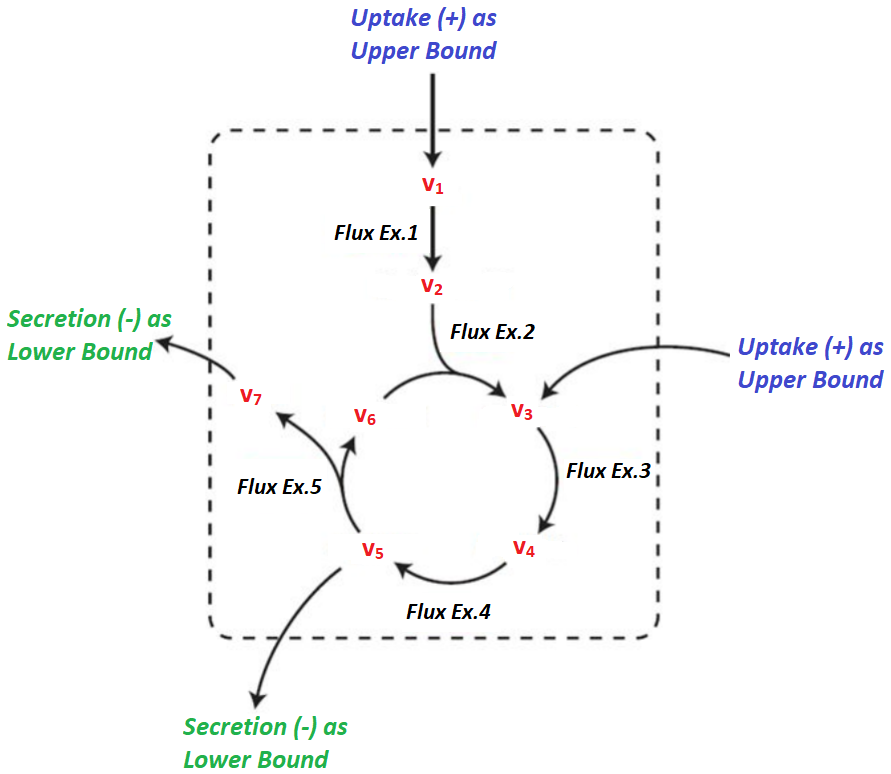
\includegraphics[width=0.57\linewidth]{../images/methodology-ORmodel-uptake_secretion_cartoon.png}}
		\caption{A Simplified Reaction-centric Network Sketch Shows The Reactions for Exchange, Uptake and Secretion.}
		\label{figure-uptake-secretion-cartoon}
	\end{center}
\end{figure}

The optimization is a linear programming problem since the mass balance (Eq.\eqref{massbalanceconstraint}), the Objective Function (Eq.\eqref{biomassmaximisation}), and the upper \& lower bounds given in Eq.\eqref{constrainedfluxlist} are structured by linear equations and the linear optimization result maximizes the structured objective function in the form of a flux distribution~\cite{KAUFFMAN2003491,PRICE2004}.

\subsection{Concept Implementation}
